\chapter{Instrument Architecture and Interfaces} \label{ch:Design}

\section{Purpose}

Digifiz Replica and Digifiz Replica Next dashboards replace the analogue instrument cluster on Volkswagen Golf Mk2, Jetta Mk2, and Scirocco Mk2 vehicles.
They deliver fully digital speed and RPM indication, LED status tell-tales, MFA trip computation, and expansion options such as Bluetooth (Replica) or Wi-Fi (Replica Next) control modules.

\section{Connector Families}

Most dashboards ship with two rectangular connectors that mate with the vehicle harness.
Replica Next variants re-use this arrangement, while certain compact versions (for example \texttt{GAC*} and \texttt{GARS*}) expose a single multipole connector.
\Cref{fig:dual-connector-layout} shows the dual-connector layout used on factory-assembled panels.

\begin{figure}[htbp]
    \centering
    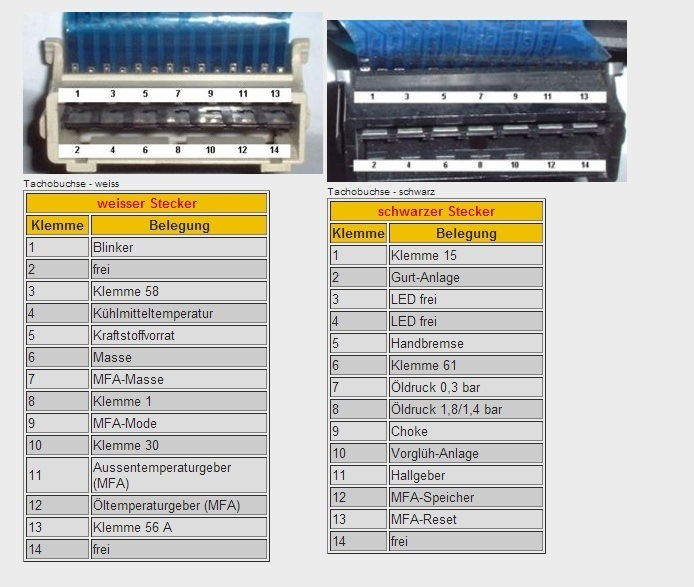
\includegraphics[width=0.8\textwidth]{digifiz_manual/image008.jpg}
    \caption{Dual-connector layout for Digifiz Replica dashboards.}
    \label{fig:dual-connector-layout}
\end{figure}

\section{White Connector Pin-out}

The white connector carries most of the low-level sensor inputs and MFA control signals.
Pin numbers follow the numbering moulded into the connector housing.

\begin{tblr}{
        colspec = {Q[c,0.12\linewidth] Q[l]},
        row{1} = {font=\bfseries},
        rowsep = 2pt,
    }
    \toprule
    Pin & Signal description \\
    \midrule
    1  & Blinker turn indicator return (pulled to ground). \\
    2  & Unused (\emph{frei}). \\
    3  & Terminal~58~+ supply for the instrument illumination. \\
    4  & Resistive coolant temperature sensor input. \\
    5  & Resistive fuel level sensor input. \\
    6  & Power ground (``mass''). \\
    7  & Power ground (``mass''). \\
    8  & Terminal~1 RPM signal (ignition coil/distributor input, accepts 0--12~V waveforms with up to 300~V spikes). \\
    9  & MFA mode selection input. \\
    10 & Permanent positive supply (``UNR''); unused on Replica, primary supply on Replica Next. \\
    11 & MFA ambient temperature sensor input. \\
    12 & MFA oil temperature sensor input (unused on Replica, enabled on Replica Next). \\
    13 & KL~56a high-beam indicator input (+12~V). \\
    \bottomrule
\end{tblr}

\section{Black Connector Pin-out}

The black connector aggregates ignition power, warning lamps, and MFA control inputs routed through the vehicle harness.

\begin{tblr}{
        colspec = {Q[c,0.12\linewidth] Q[l]},
        row{1} = {font=\bfseries},
        rowsep = 2pt,
    }
    \toprule
    Pin & Signal description \\
    \midrule
    1  & Terminal~15 ignition-switched positive supply. \\
    2  & Not connected. \\
    3  & Not connected. \\
    4  & Not connected. \\
    5  & Handbrake warning lamp (active when grounded). \\
    6  & KL~61 generator warning lamp with 120~\ohm{} excitation resistor at +12~V. \\
    7  & Oil pressure switch, 0.3~bar threshold. \\
    8  & Oil pressure switch, 1.8~bar threshold. \\
    9  & Not used. \\
    10 & Glow-plug indicator lamp (diesel variants, active at +12~V only). \\
    11 & Hall sensor input for the electronic speed sensor (via diode on request). \\
    12 & MFA memory block selection input. \\
    13 & MFA reset input. \\
    \bottomrule
\end{tblr}

\section{Single-Connector Variants}

Some panels consolidate the wiring into a single multipole connector.
\Cref{fig:single-connector} summarises the pin layout; the detailed assignments follow the same numbering as the dual-connector design.

\begin{figure}[htbp]
    \centering
    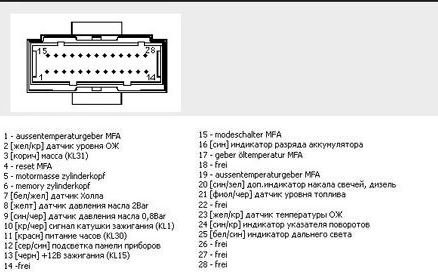
\includegraphics[width=0.72\textwidth]{digifiz_manual/image009.png}
    \caption{Single-connector layout for compact Digifiz Replica variants.}
    \label{fig:single-connector}
\end{figure}

\section{Scirocco Harness Pin-out}

Prospective Scirocco harnesses use a five-pin auxiliary connector and a fourteen-pin main connector.
The mapping below follows the documentation bundled with the experimental harnesses.

\begin{tblr}{
        colspec = {Q[c,0.12\linewidth] Q[l] Q[c,0.12\linewidth] Q[l]},
        row{1} = {font=\bfseries},
        rowsep = 2pt,
    }
    \toprule
    \multicolumn{2}{c}{5-pin connector} & \multicolumn{2}{c}{14-pin connector} \\
    Pin & Signal & Pin & Signal \\
    \midrule
    1 & D3 & 1  & KL58 (illumination) \\
    2 & D2 & 2  & MASS (ground) \\
    3 & D1 & 3  & TANK (fuel level) \\
    4 & SA & 4  & TEMP (coolant sensor) \\
    5 & SPERRE & 5  & KL1 (RPM) \\
    6 & SSA & 6  & UHR (permanent +12~V) \\
    -- & -- & 7  & FERNL (high beam) \\
    -- & -- & 8  & Auxiliary, reserved \\
    -- & -- & 9  & OEL~1.8 (oil pressure, high) \\
    -- & -- & 10 & CAT~VORGL$(-)$ (diesel pre-heater) \\
    -- & -- & 11 & OEL~0.3 (oil pressure, low) \\
    -- & -- & 12 & KL61 (generator lamp) \\
    -- & -- & 13 & KL49A (indicator feed) \\
    -- & -- & 14 & KL15 (ignition +12~V) \\
    \bottomrule
\end{tblr}

\section{Mk1 Connector Mapping}

For Mk1 conversions, the fourteen-pin connector follows the mapping below.
The diagram in \Cref{fig:mk1-wiring} illustrates the physical layout.

\begin{enumerate}
    \item Illumination and low-beam feed.
    \item MASSE~31 (vehicle ground).
    \item TANK (fuel level sensor).
    \item TEMP (coolant temperature sensor).
    \item KL~1 (RPM signal).
    \item UHR (permanent +12~V).
    \item KL~56 (high beam input).
    \item OIL~(HIGH) 1.8~bar sensor.
    \item OIL~(LOW) 0.3~bar sensor.
    \item Diesel glow-plug indicator.
    \item CHOKE (not used).
    \item KL61 generator warning lamp.
    \item Combined indicator output (left/right blinkers).
    \item KL15 ignition-switched +12~V.
\end{enumerate}

\begin{figure}[htbp]
    \centering
    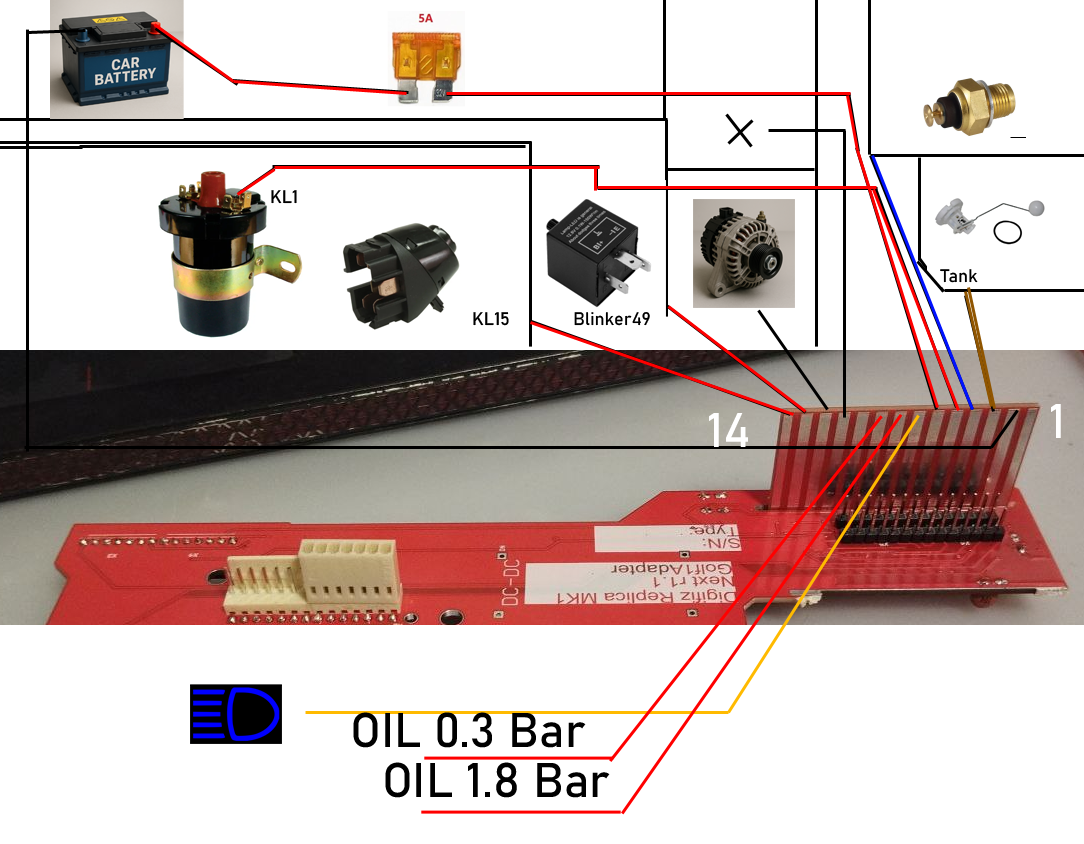
\includegraphics[width=0.75\textwidth]{digifiz_manual/image010.png}
    \caption{Mk1 harness connector layout.}
    \label{fig:mk1-wiring}
\end{figure}

\section{Service Connector}

A fourteen-pin service connector provides direct access to diagnostic signals, auxiliary indicators, and optional inputs.
Pin numbers are counted from right to left when viewing the dashboard from the rear, matching the original Digifiz numbering.
\Cref{tbl:service-connector} lists the assignments and highlights the differences between Replica and Replica Next.

\begin{tblr}{
        colspec = {Q[c,0.12\linewidth] Q[l]},
        row{1} = {font=\bfseries},
        rowsep = 2pt,
    }
    \toprule
    Pin & Signal description \\
    \midrule
    1  & Indicator output. \\
    2  & Speed sensor input (signal~\#2, SPM\textsubscript{M}). \\
    3  & Vehicle ground. \\
    4  & Indicator output. \\
    5  & Optocoupler input for the left turn signal. \\
    6  & Optocoupler input for the right turn signal. \\
    7  & +12~V supply from ignition. \\
    8  & Diesel-specific input. \\
    9  & Indicator input (positive). \\
    10 & Alternate RPM input (reserved; currently unused on Replica Next). \\
    11 & Replica: indicator feed normally routed to the optocoupler; Replica Next: brake indicator (low-side). \\
    12 & Reserved input. \\
    13 & Check-engine input. \\
    14 & No connection. \\
    \bottomrule
\end{tblr}

\begin{figure}[htbp]
    \centering
    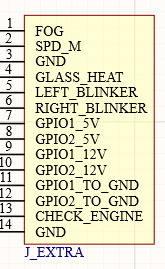
\includegraphics[width=0.7\textwidth]{digifiz_manual/image013.png}
    \caption{Service connector orientation on the Replica PCB.}
\end{figure}

\section{Firmware Resources}

The complete firmware and hardware design files are published at\newline\url{https://github.com/Sgw32/DigifizReplica}.
The repository hosts the Arduino-based firmware for Digifiz Replica as well as the ESP32-based firmware for Replica Next.
